\chapter{Vertex Reconstruction}

In the next decade, the planned High Luminosity Large Hadron Collider (HL-LHC) upgrade~\cite{Apollinari:2284929} will enhance our experimental sensitivity to rare phenomena by increasing the number of collected proton-proton collisions by a factor of ten. The average number of pileup events per interaction is expected to rise from 40 to over 100. This high-luminosity environment will produce a new set of challenges for track and vertex reconstruction, requiring major upgrades in both hardware and in reconstruction algorithms.

As part of my ATLAS authorship project, I conducted a set of vertex reconstruction algorithm studies, which I presented at a Winter 2015 workshop in Chamonix. Note that since it has been several years since then, the studies shown here may be out of date.

The basic vertex reconstruction method is as follows. First, we perform seed finding, where we tag locations along the beam axis that are likely vertex candidates. This is typically performed using a simple clustering algorithm. After this, we associate all tracks in the event with their nearest vertex seed. The tracks associated with each seed are then used to reconstruct the exact location of the vertex.

Grading our algorithm is a multi-step process. First we look at which truth vertex each reconstructed track is coming from. Each track has a weight associated, which is a measure of how certain we are that the track was reconstructed correctly. A track could be reconstructed properly (meaning that it corresponds to some degree with a truth track), or it could be completely misconstructed, in which case we call it a fake track.

Next, we look at the reco tracks which we've associated with each reco vertex. If two or more reco vertices have their largest track weight contributions coming from a single truth vertex, the truth vertex is considered to be split. If a reco vertex has more than $70\%$ of its track weight coming from a single truth vertex, and the truth vertex is not split, we say that the reco and truth vertices are matched. If no truth vertex contributes more than $70\%$ track weight to a reco vertex, and the contributing truth vertices are not split, the reco vertex is considered merged. Finally, if there is more track weight from fake tracks than from any truth vertex in a reco vertex, the reco vertex is considered fake.

Finally, we consider the hard scatter (HS) vertex, which is defined as the vertex with the greatest sum \pt\ of decay products. If the HS truth vertex contributes more than $70\%$ track weight to a single reco vertex, and the HS vertex contributes the majority of track weight to only a single reco vertex, the HS reconstruction is considered clean. If the HS vertex contributes majority of track weight for a single vertex, but the weight adds up to less than $70\%$ of that vertex's total track weight, the event is considered low-pileup. If the HS contributes any track weight to any reco vertex, but is not the highest track weight component for any of them, the event is considered high-pileup. If there is more than one reco vertex for which the HS contributes the most track weight, the event is considered split. And finally, if there are no vertices with any HS components at all, the event is considered a no match.

It has been shown through simulations of high-pileup environments that we begin to see unacceptable levels of vertex merging, as well as an increasing number of HS classifications which are low-pileup or high-pileup. For this reason, we investigated the use of a new seed-finding and vertex reconstruction algorithm. The studies here are shown with current pileup conditions, though studies have since been performed using the proposed pileup environment.

In this algorithm, we begin by filling a voxelated region of space with our reconstructed tracks. This 3D image is then sent through a fast Fourier transform, a frequency filter is applied to remove high-frequency components, and the result is sent through a reverse transform, as seen in Figure~\ref{fig:FFT}.

\begin{figure}[htbp]
    \centering
    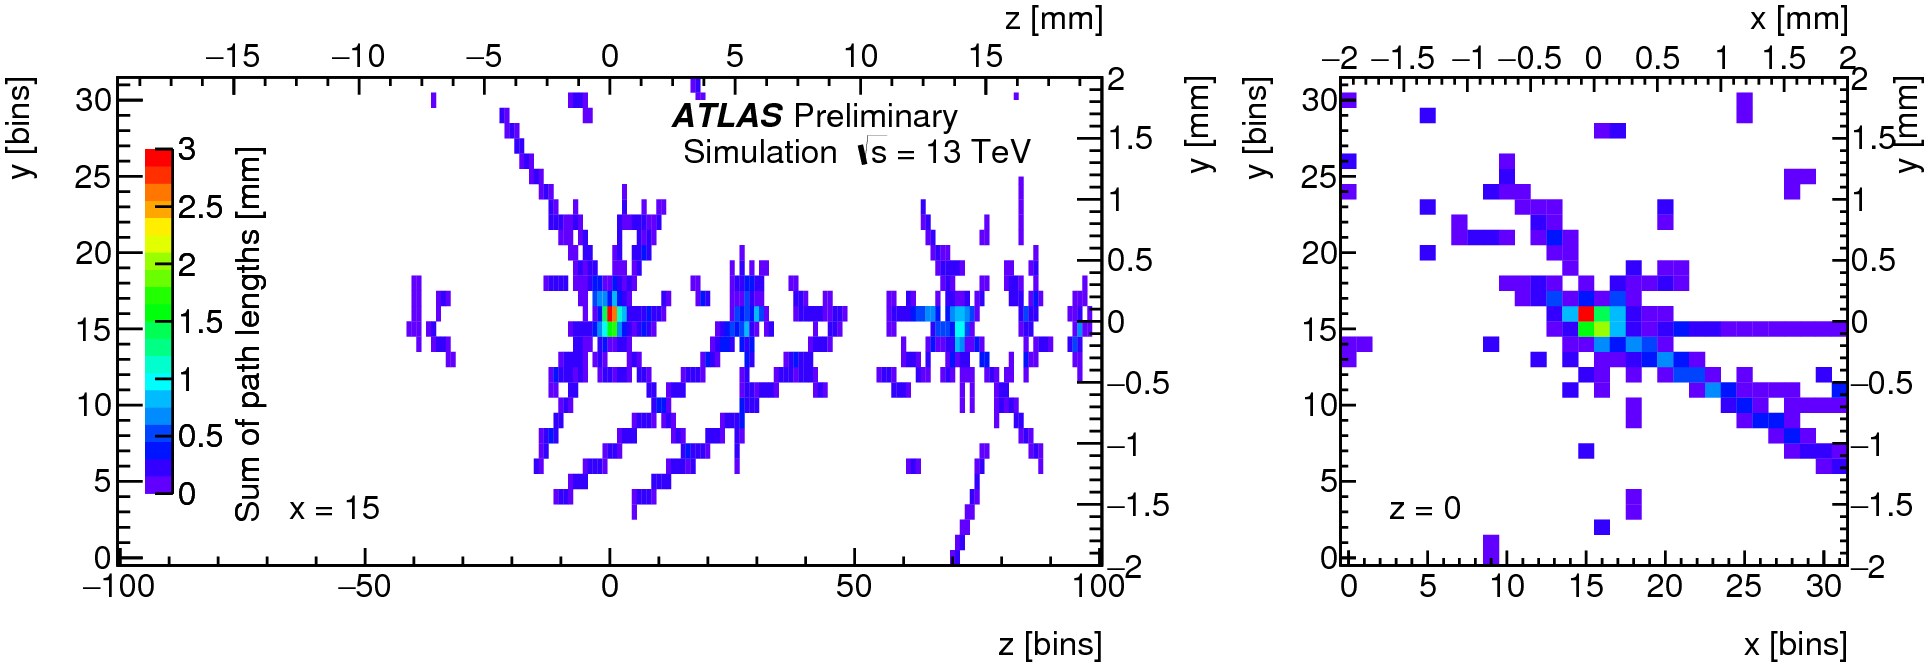
\includegraphics[width=\linewidth]{Images/Other/vertex_FFT_1.png}
    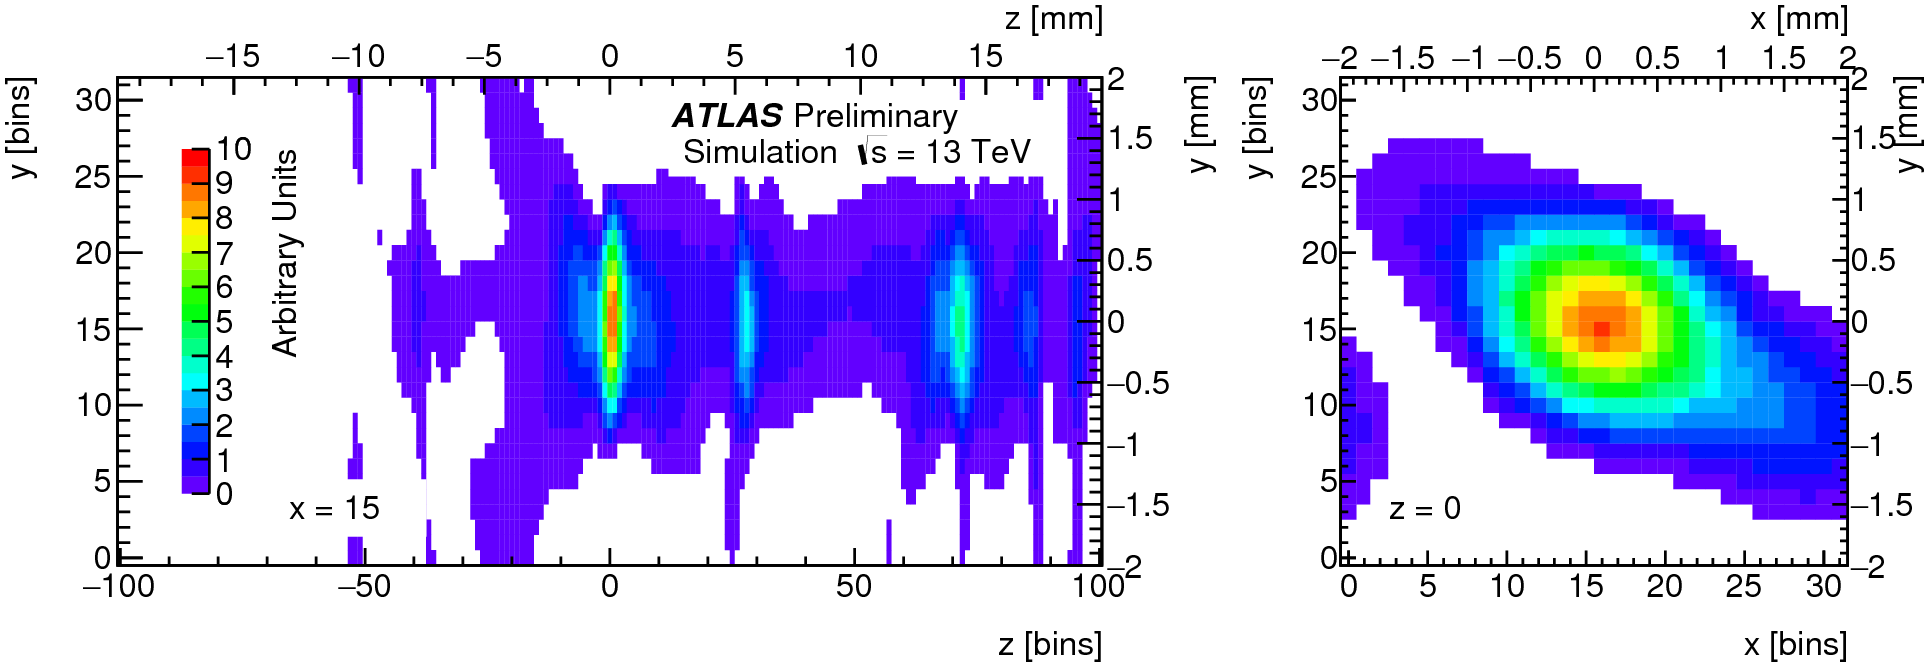
\includegraphics[width=\linewidth]{Images/Other/vertex_FFT_2.png}
    \caption{Voxelated tracks (top), and the result of a frequency filter applied to an FFT (bottom).}
    \label{fig:FFT}
\end{figure}

This result is then collapsed onto the beam axis (z-axis), as seen in Figure~\ref{fig:seeds}. Here, all local maxima above a certain threshold are marked as seeds, or potential vertices. Tracks are then associated with their nearest seeds, and vertices are reconstructed. The results of seed-finding are shown in Figure~\ref{fig:seed_comparison}.

\begin{figure}[h]
    \centering
    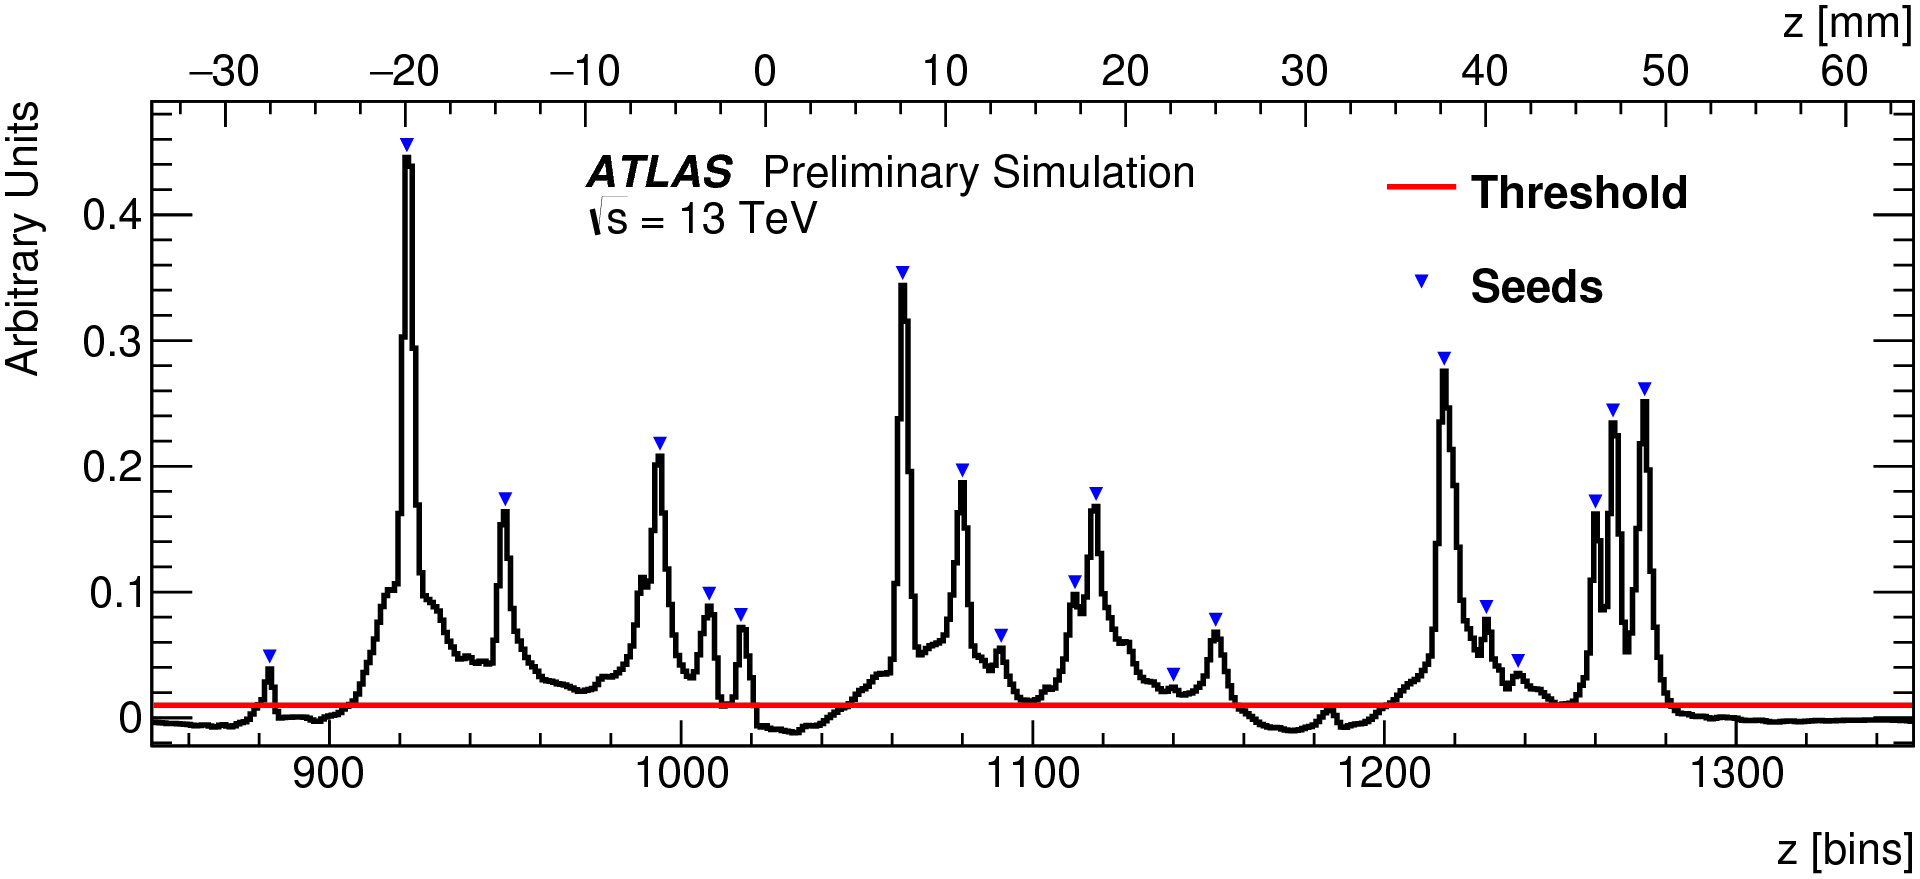
\includegraphics[width=0.9\linewidth]{Images/Other/seeds.png}
    \caption{Result of FFT collapsed on the beam axis. Local maxima above a threshold are identified as vertex seeds.}
    \label{fig:seeds}
\end{figure}

\begin{figure}[h]
    \centering
    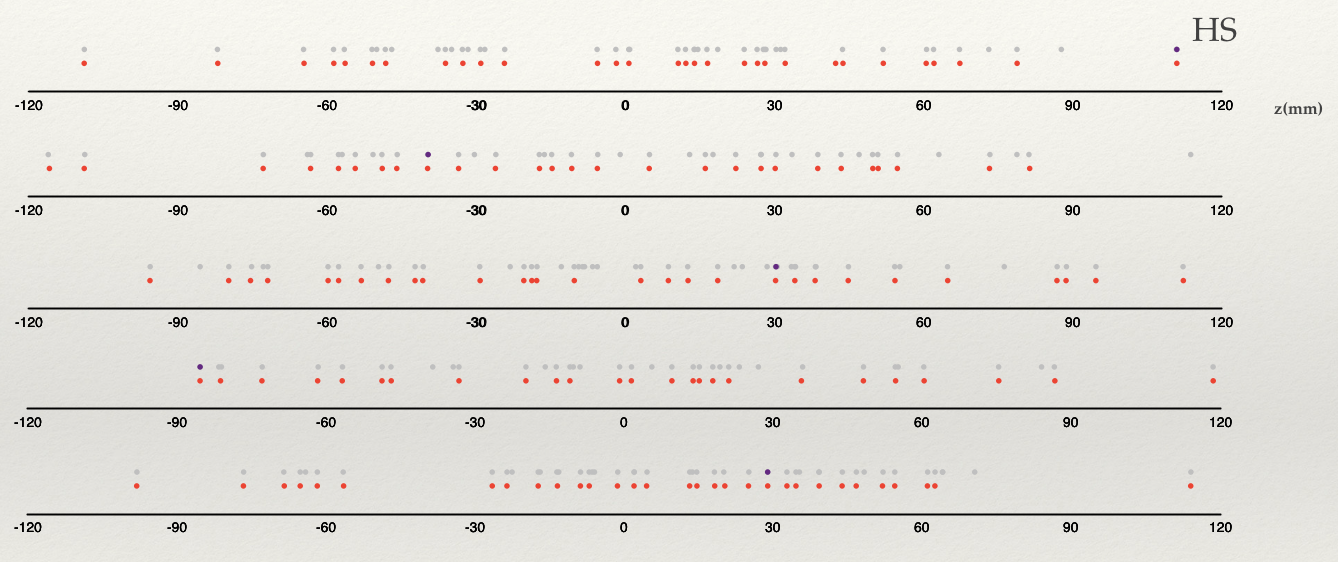
\includegraphics[width=\linewidth]{Images/Other/seed_comparison.png}
    \caption{Results of seed-finding. Seeds in red are compared with truth vertices in gray. Hard scatter vertices are in purple.}
    \label{fig:seed_comparison}
\end{figure}

We compare the results of this seed-finding technique against the previously-used technique in Figure~\ref{fig:seed_method_compare}. The new method finds more vertices overall, but splitting is more of an issue. This can also be seen in Figure~\ref{fig:vertices_compare}.

\begin{figure}[H]
    \centering
    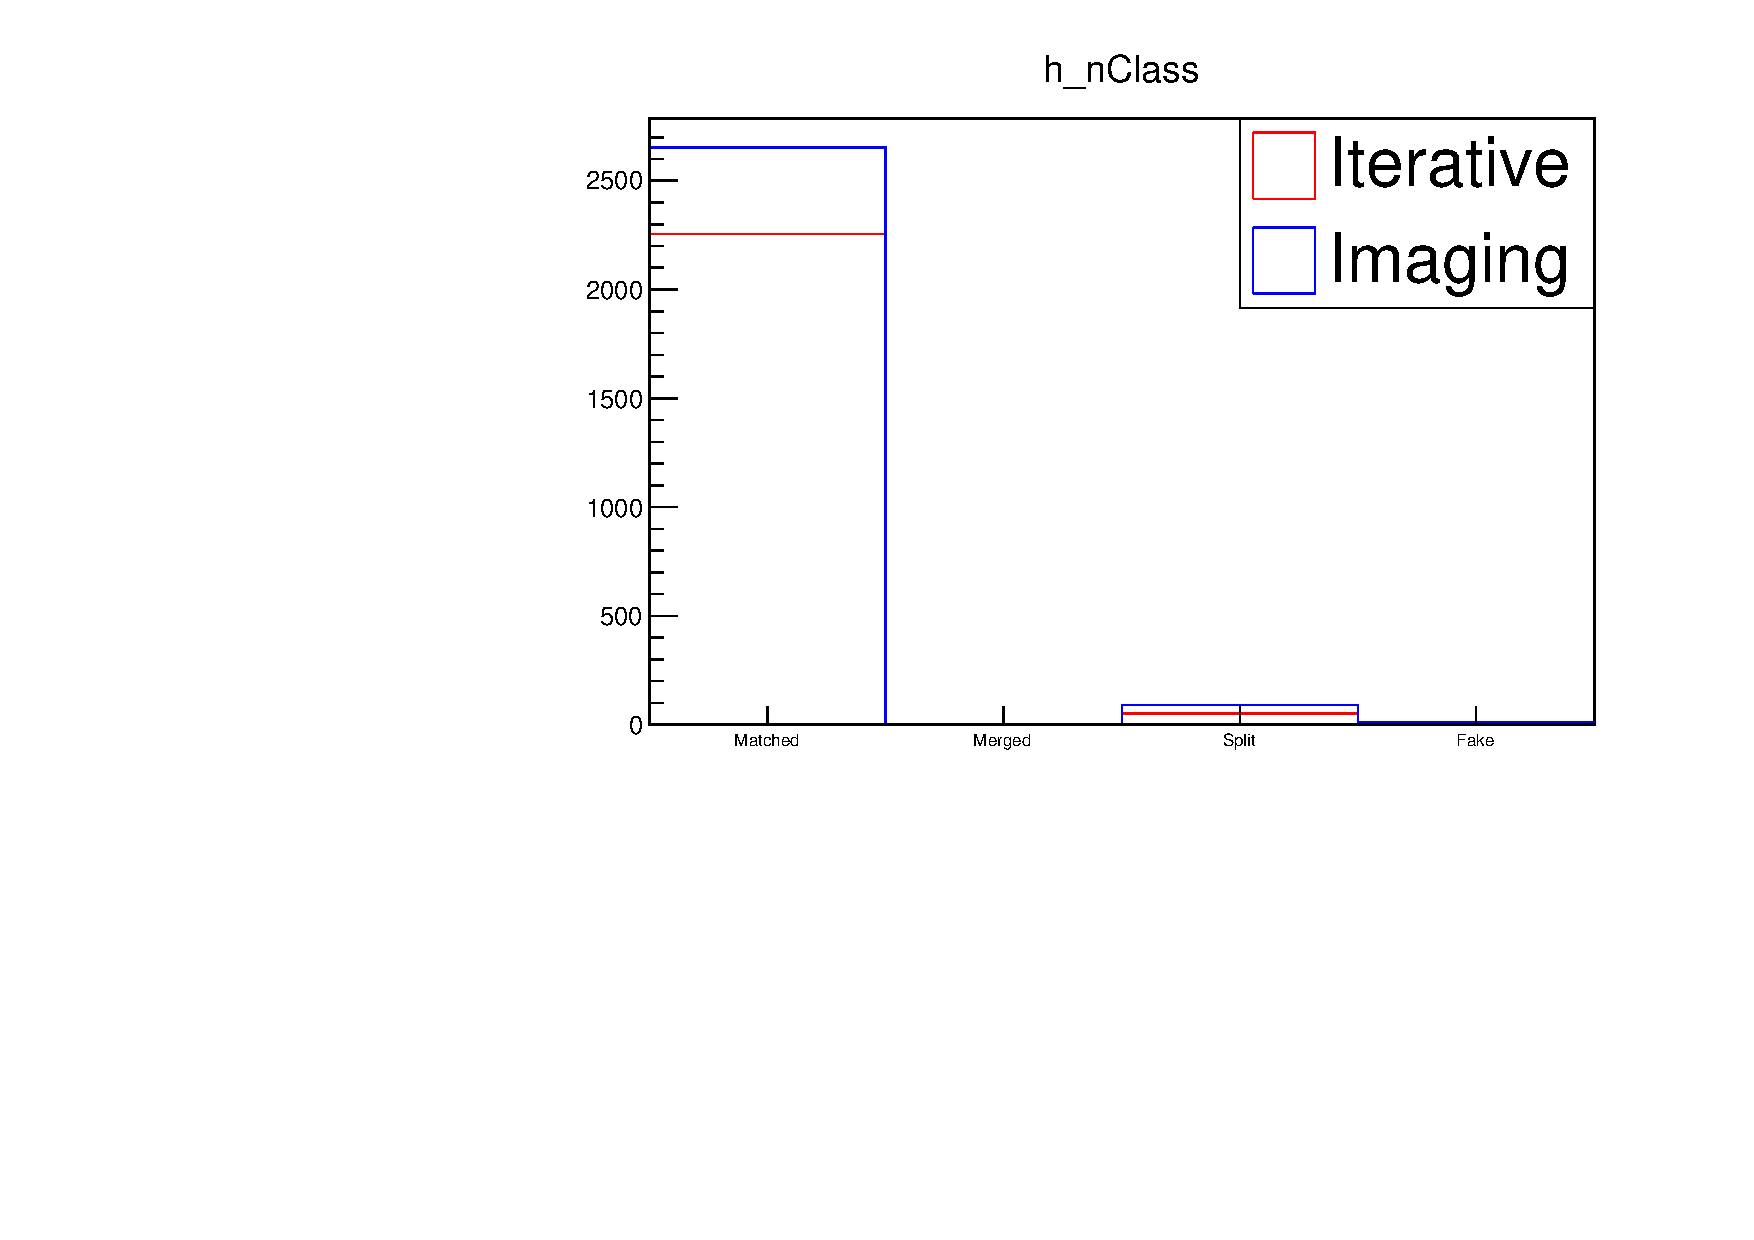
\includegraphics[width=0.45\linewidth]{Images/Other/h_nClass.pdf}
    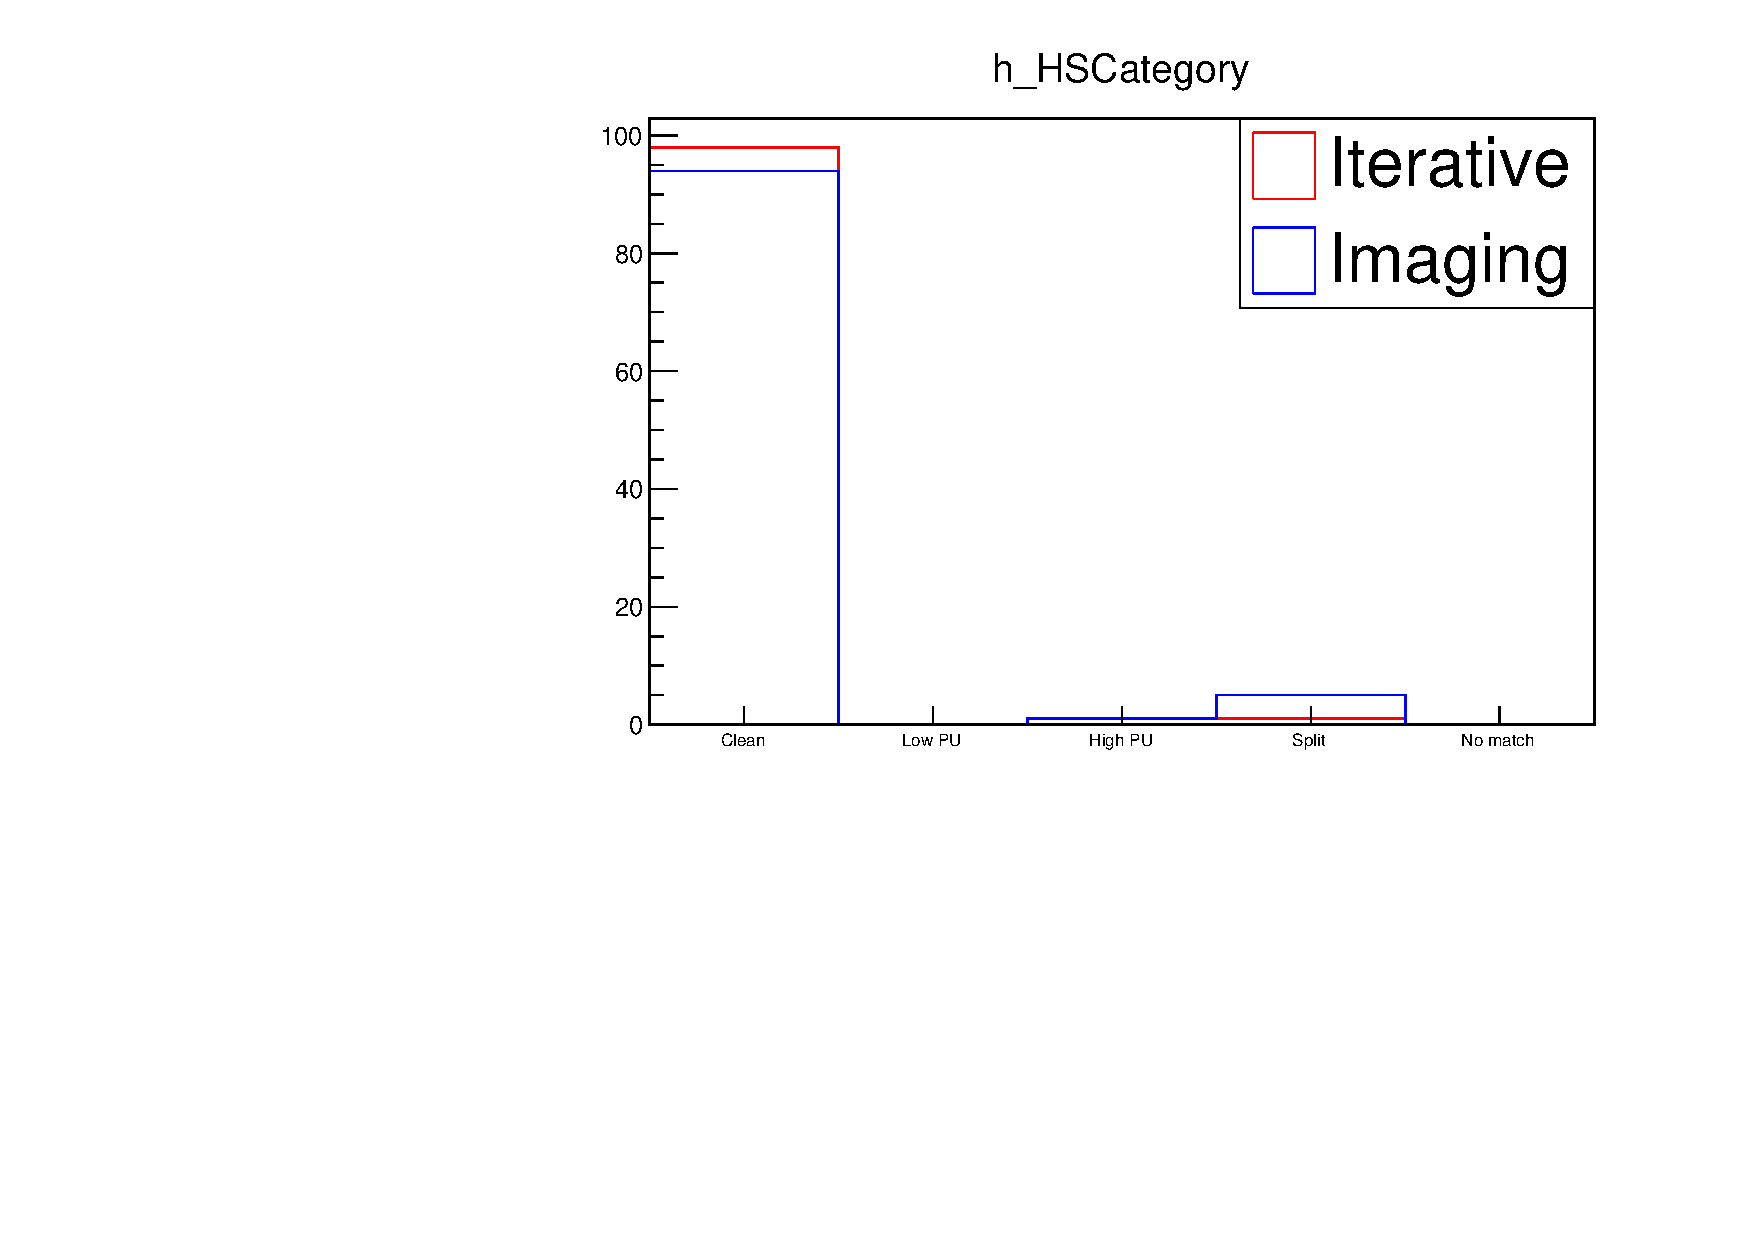
\includegraphics[width=0.45\linewidth]{Images/Other/h_HSCategory.pdf}
    \caption{Comparison of the algorithm described here (imaging) vs. the previously-used algorithm (iterative). On the left we see classification results for all vertices, and on the right we see results for hard scatter vertices.}
    \label{fig:seed_method_compare}
\end{figure}

\begin{figure}[htbp]
    \centering
    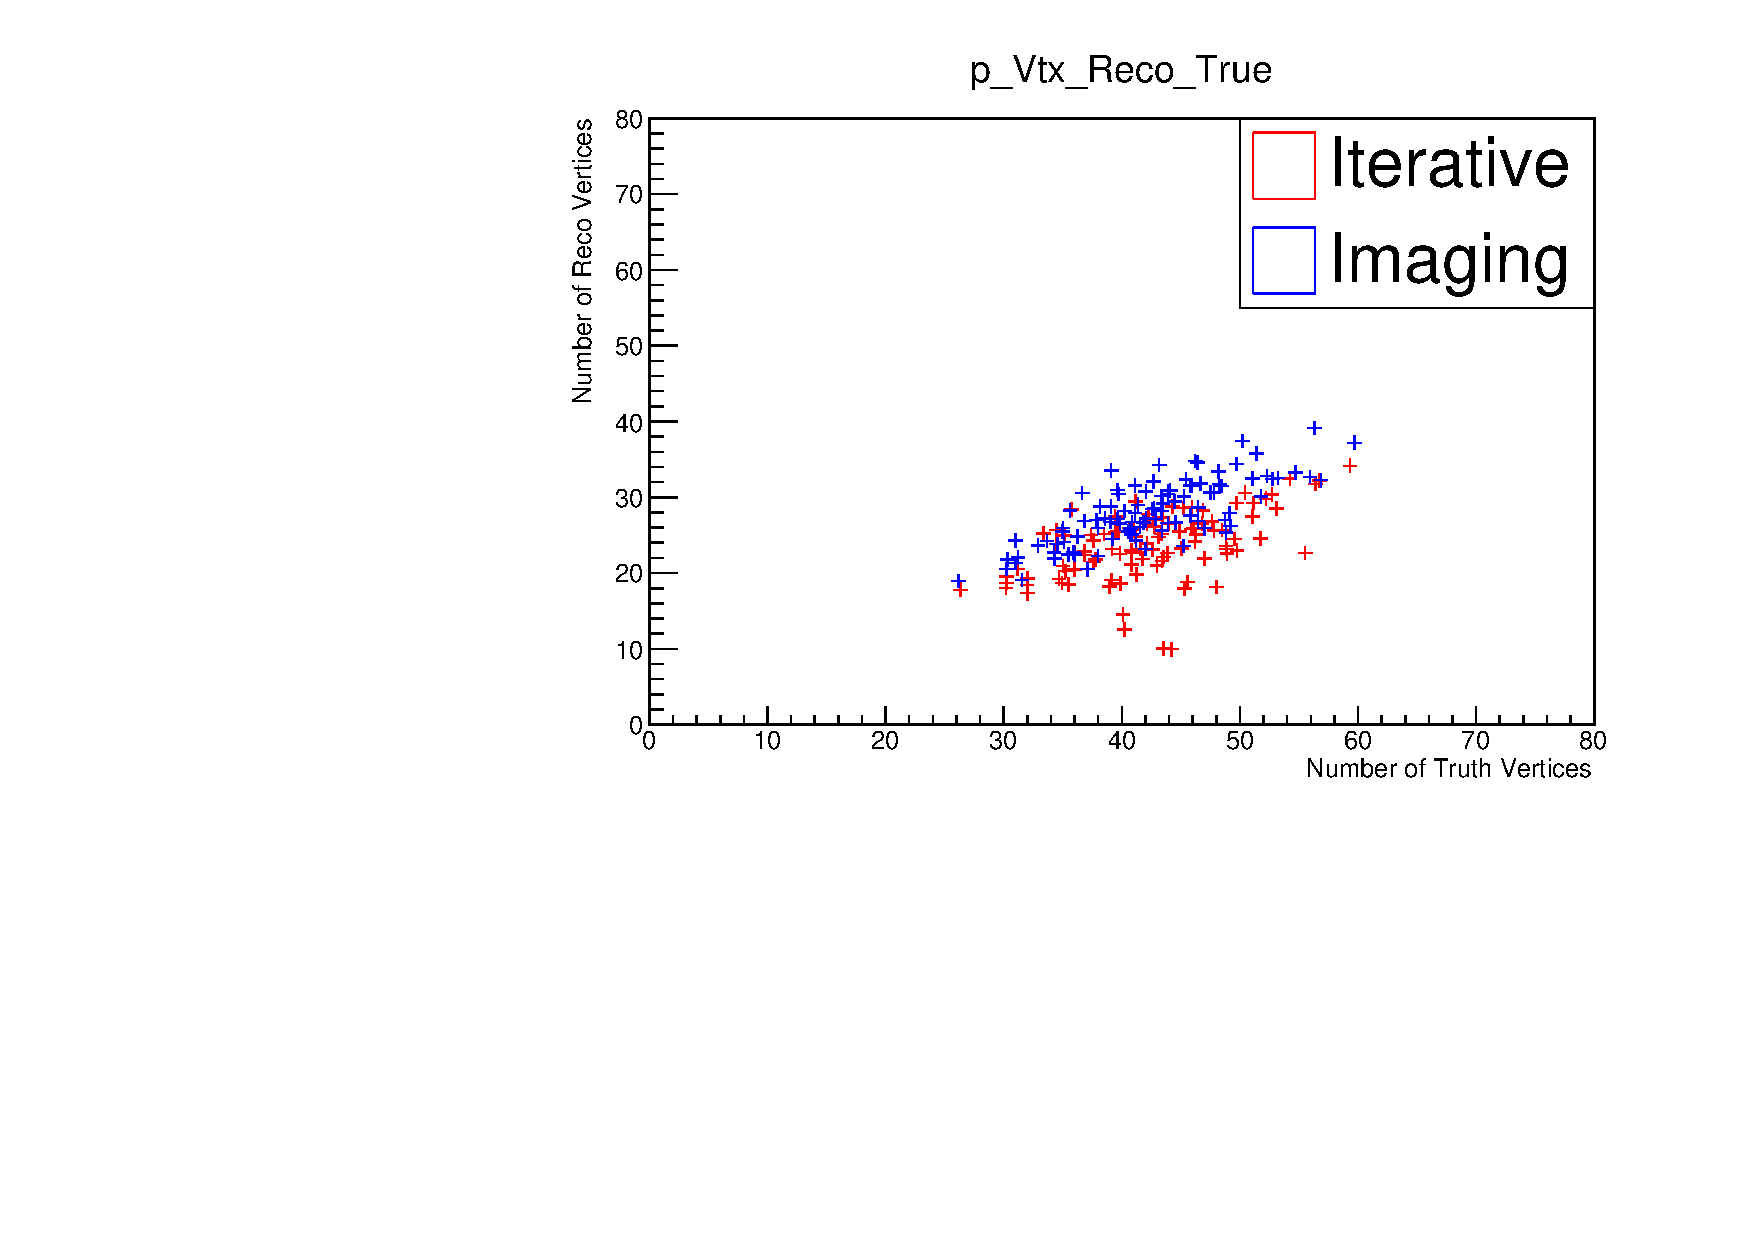
\includegraphics[width=0.7\linewidth]{Images/Other/p_Vtx_Reco_True.pdf}
    \caption{Comparison of two seed-finding algorithms. The algorithm described here is labeled "imaging", while the previously-used algorithm is labeled "iterative".}
    \label{fig:vertices_compare}
\end{figure}

A few examples of reconstructed vertices after track association can be seen in Figure~\ref{fig:track_association}. In order to improve reconstruction, I also tried a machine learning algorithm for associating tracks with seeds, rather than just using the nearest one. This approach did not really help with the splitting issue, so the overall improvement was not large. After I completed my authorship project, the vertex reconstruction group continued to work on the problem in anticipation for the coming luminosity upgrade.

\begin{figure}[htbp]
    \centering
    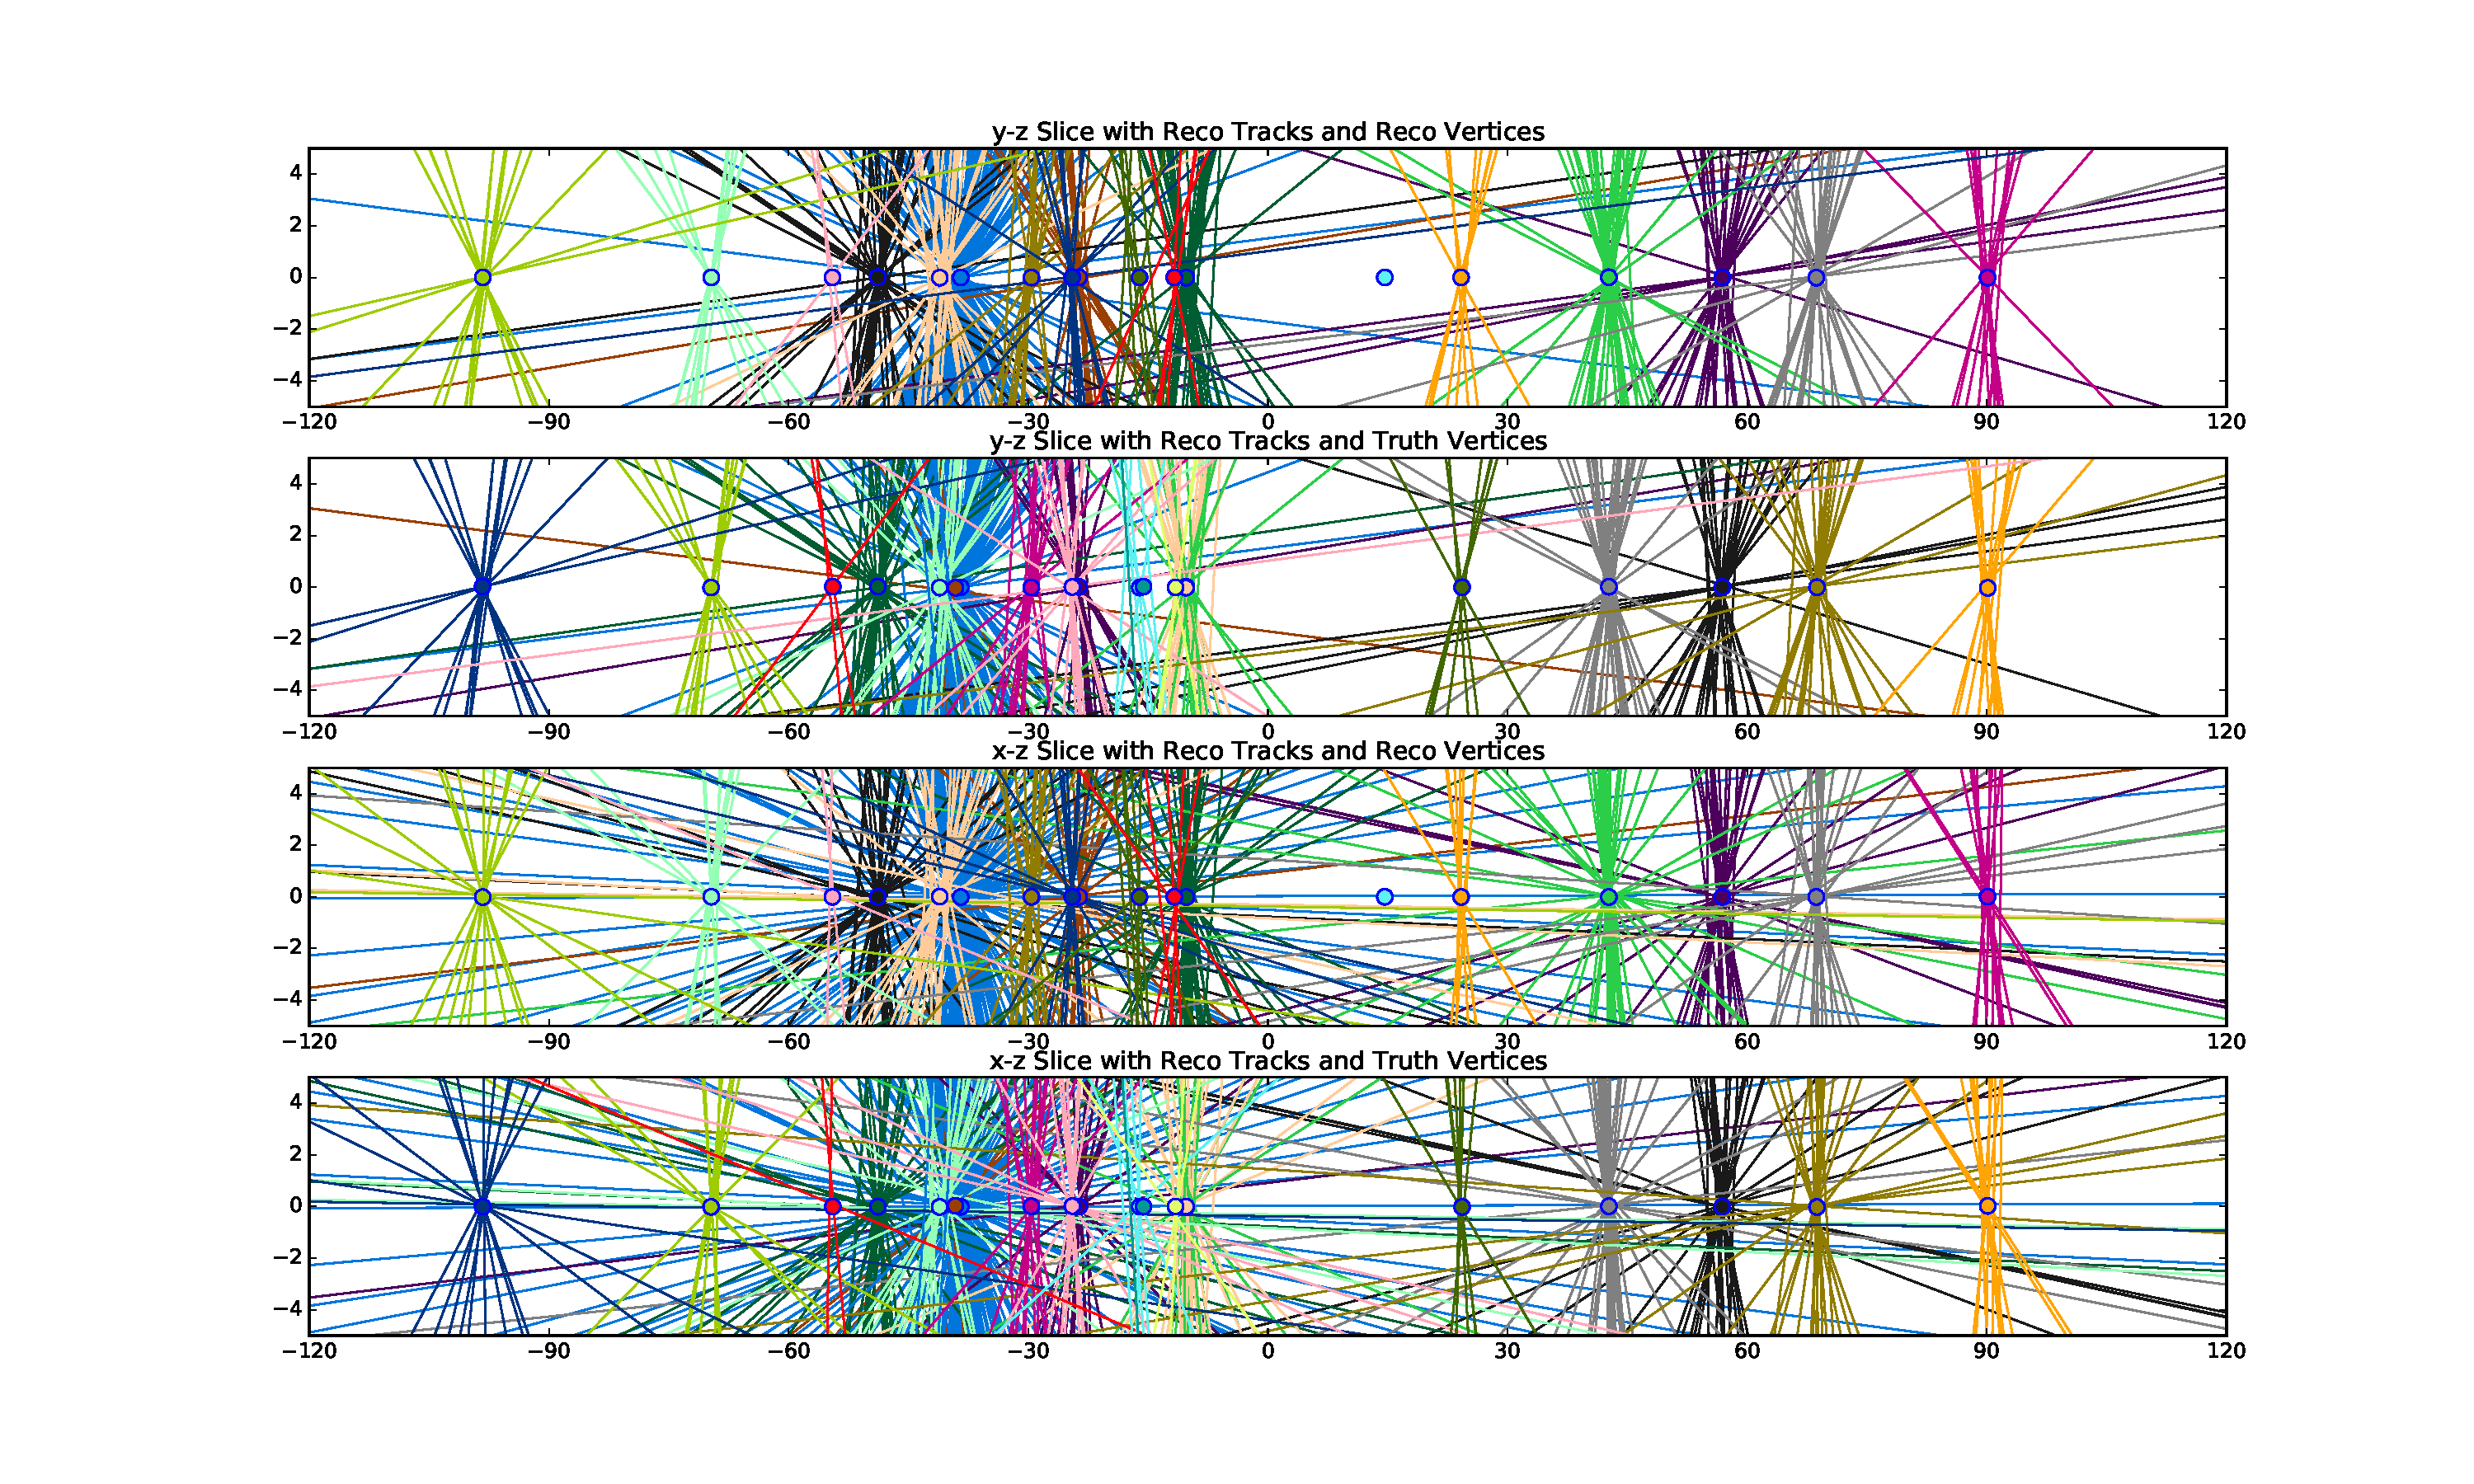
\includegraphics[trim=120 70 120 70, clip, width=\linewidth]{Images/Other/track_association.pdf}
    \caption{Reconstructed vertices after track association. Truth vertices are shown as colored dots, while reconstructed vertices are shown via their associated tracks, as colored lines.}
    \label{fig:track_association}
\end{figure}